\documentclass{jarticle}
\usepackage[dvipdfmx]{graphicx}
\usepackage{here}
\usepackage{listings,jlisting}


\lstset{
  basicstyle={\ttfamily},
  identifierstyle={\small},
  commentstyle={\smallitshape},
  keywordstyle={\small\bfseries},
  ndkeywordstyle={\small},
  stringstyle={\small\ttfamily},
  frame={tb},
  breaklines=true,
  columns=[l]{fullflexible},
  numbers=left,
  xrightmargin=0zw,
  xleftmargin=3zw,
  numberstyle={\scriptsize},
  stepnumber=1,
  numbersep=1zw,
  lineskip=-0.5ex
}

\title{{システム実験}\\基礎実験4レポート}
\author{6119019056 山口力也}
\date{2019/05/17日提出}

\begin{document}
\maketitle
\section{基礎実験第4回の概要}
基礎実験第4回目の実験の目的,実施した実験の概要,および理解した事柄を100~200字程度で説明せよ.

\subsection{実験目的}
以下の示す事柄を実験目的とした.

\begin{itemize}

\item 割り込みの動作原理を知る.
\item ポーリングと割り込みの処理の違いを理解する.
\item タイマ割り込みの動作原理を理解して使いこなせる.
\item 外部割り込みの動作原理を理解して使いこなせる.

\end{itemize}

\subsection{実験概要}
実験内容としてマイコンを用いた割り込み処理として"タイマ割り込み"と"外部割り込み"を扱った.

\subsection{理解した事柄}
マイコンのプログラムをより効率的に実行する割り込み機能の動作原理を理解し,実装方法を習得し理解した.

\section{回路実装}
基礎実験4で使用した回路のブレッドボード配線図を報告せよ.

以下\ref{fig:bread}に使用した回路のブレッドボード配線図を示す.

\begin{figure}[H]
\begin{center}
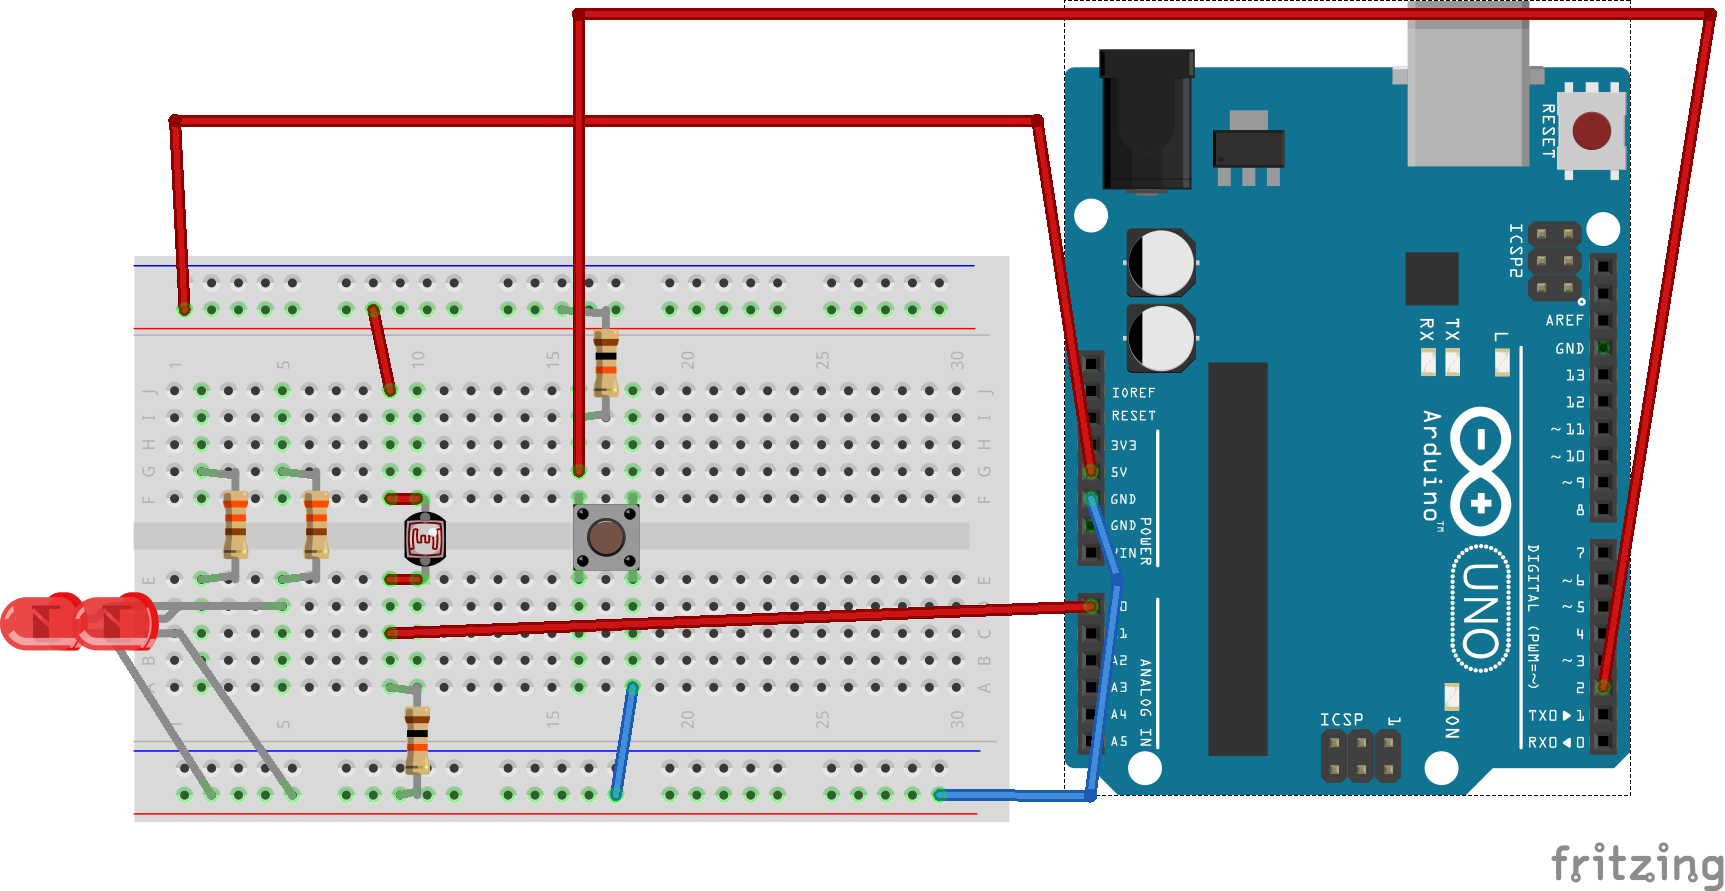
\includegraphics[width=7.0cm]{images/bread.png}
\caption{基礎実験4で使用した回路の配線図}
\label{fig:bread}
\end{center}
\end{figure}

\section{タイマ割り込みによるLEDの点滅}
課題2.4.1において作成したスケッチおよび完成させた図2.63を報告せよ.また,MsTimer2を使用せずにポーリング処理のみを使用した場合どのような問題点があるのか調査し,報告せよ.

以下ソースコード\ref{code:kadai2-4-1}に作成したスケッチを示す.

\begin{lstlisting}[caption = 課題2.4.1,label=code:kadai2-4-1][H]
#include <MsTimer2.h>
const int LED1_PIN = 13; //13番ピンにLEDを接続
const int LED2_PIN = 9; //9番ピンにLEDを接続

void flash() { //割り込みサービスルーチン(LEDの点滅)
  for ( int i = 255; i >= 0 ; i--){ //発光状態から消灯状態へ
    analogWrite(LED2_PIN,i); //LED2_PINにPWM出力
    delay(5000/256); //256回(発光->消灯間5000ms)
  }
  
}

void setup() {
  pinMode(LED1_PIN, OUTPUT); //13番ピンを出力ポートに設定
  pinMode(LED2_PIN,OUTPUT); //9番ピンを出力ポートに設定
  MsTimer2::set(20, flash); // タイマ割り込み間隔の設定(500ms)
  MsTimer2::start(); //タイマ割り込み開始
}

void loop() { //ボーリング処理
  digitalWrite(LED1_PIN,HIGH); //13番ピンに5V出力
  delay(500); //500ms待機
  digitalWrite(LED1_PIN,LOW); //13番ピンに0V出力
  delay(500); //500ms待機
}
\end{lstlisting}

また,以下図\ref{fig:2-63}に完成させた図2.63を示す.

\begin{figure}[H]
\begin{center}

\includegraphics[width=7.0cm]{images/figure2-63.png}
\caption{周期の異なるLEDの同時点滅}
\label{fig:2-63}
\end{center}
\end{figure}

MsTimer2を使用せずにポーリング処理のみを使用した場合は,20msごとに呼び出される割り込みに500ms待機が入っているので,うまく割り込めず500msずつ処理がずれていくと思われる.

\section{タイマ割り込みによる照度センサのデータ取得}
課題2.4.2において作成したスケッチを報告せよ.また,「手で光を遮る」「光を遮らない」状態を素早く繰り返した時に生じた取りこぼしについて原因を考察せよ.さらに,取りこぼしを回避する方法案を記せ.

以下ソースコード\ref{code:kadai2-4-2}に作成したスケッチを示す.


\begin{lstlisting}[caption = 課題2.4.2,label=code:kadai2-4-2][H]
unsigned long timePrev = 0; //基準となる時間を格納

void check() {
  static int sensorvalue = analogRead(A0); //A0ピンのAD変換結果を取得
  Serial.println(sensorvalue);
}
void setup() {
  Serial.begin(9600); //シリアル通信を9600kbpsで初期化
  pinMode(13,OUTPUT); //13番ピンを出力ポートに設定
}

void loop() { //millis関数による時間計測
  unsigned long timeNow = millis(); //millis関数を用いて現在の時間情報を取得
  if(timeNow - timePrev >= 500){ //500ms以上経過
    check(); //check関数の処理を実行
    timePrev = timeNow; //時間情報の更新
  }
  else{}
}
\end{lstlisting}
「手で光を遮る」「光を遮らない」状態を素早く繰り返した時に生じた取りこぼした原因は,mills関数の値にある.500msごとにセンサの値を読み取っているため500msの間にあった変化に関してはセンサは読み込めない.取りこぼしを回避するにはmills関数の値をより小さくして細かくセンサの値を読み取る必要があるが,細かくしすぎると値を読み取る回数が増えて処理が重くなる.

\section{スイッチ動作の外部割り込みによるLEDの点灯・消灯}
演習2.4.5において生じるチャタリングについて調査し報告せよ.また,attachInterruptを使用せずにポーリング処理のみを使用した場合,どのような問題が生じるのか調査し,報告せよ.

チャタリングとは,物理的なスイッチなどを使用した時,スイッチを押した瞬間にONとOFFの状態が非常に短い間隔で振動することである.今回の実験では物理スイッチを用いているため,ONにした瞬間にONとOFFが交互に動作して誤動作を起こしている.\\
また,attachInterruptを使用せずにポーリング処理のみを使用した場合,ループ関数の中で処理を定義する必要がある.ループ関数で処理を行っている途中に外部割り込みがあった場合,外部割り込みを認識できないか,反応が遅れる..またループ処理の中で信号を検知する場合,常に信号があるかないかを確認する必要があるので処理が多くなる.
\section{スイッチ動作に外部割り込みによるLED発行のフェイドイン・フェイドアウト}
課題2.4.3で作成したスケッチを報告せよ.またスケッチで工夫した点を工夫せよ.

以下ソースコード\ref{code:kadai2-4-3}に作成したスケッチを示す.

\begin{lstlisting}[caption = 課題2.4.3,label=code:kadai2-4-3][H]
const int LED_PIN = 9; //LEDをD9に定義
volatile int flag = LOW; //フェードイン,フェードアウト判定用の変数を用意
int i = 0;
unsigned long timePrev = 0;//時間を格納
/* 初期設定 */
void setup() {
  pinMode(LED_PIN,OUTPUT); //D9を出力に設定
  /*外部割り込みの設定
    割り込みに使用するディジタルポートをD2に設定(1番目の引数="0")
    割り込みサービスルーチンblink関数を実行(2番目の引数=関数名)
    (例)割り込み要因としてスイッチの状態が"LOW"のときに発生(3番目の引数)
   */
   attachInterrupt(0,blink,FALLING);
}

void loop() {
  if ( flag == LOW ){
    if( i == 255 ){
      i = 0;
    }
    analogWrite(LED_PIN,i);
    i++;
	 timePrev = millis();
	 while(millis() - timePrev <= 3000/255){
		 //3000/255秒待つ
	 }
  }
   else{
    if( i == 0 ){
      i = 255;
    }
    analogWrite(LED_PIN,i);
    i--;
	 timePrev = millis();
	 while(millis() - timePrev <= 3000/255){
		 //3000/255秒待つ
	 }
  }
}
void blink() { //割り込みの条件にあわせLEDがフェードイン・フェードアウトを繰り返す
  flag = !flag;
}
\end{lstlisting}

スケッチで工夫した点は,スイッチが押された時ようにflagを用意しておき,flagが変更したらそれぞれ加算か減算のfor文に入るようにif文で制限したところである.


\section{発展課題2.4.1}
発展課題2.4.1において作成したスケッチと工夫点を報告せよ.また,照度センサの値の変化をグラフ化し,その結果を報告せよ.

以下ソースコード\ref{code:hatten2-4-1}に作成したスケッチを示す.

\begin{lstlisting}[caption = 発展課題2.4.1,label=code:hatten2-4-1][H]
#include <MsTimer2.h>
const int LED1_PIN = 13; //13番ピンにLEDを接続
const int LED2_PIN = 9; //9番ピンにLEDを接続
volatile int flag = 0; //10秒経過flag
int output = LOW;
unsigned long timePrev10 = 0; //基準となる時間を格納(10秒用)
unsigned long timePrev500 = 0; //基準となる時間を格納(500ms用)
void check() { //割り込みサービスルーチン(LEDの点滅)
  int sensorvalue = analogRead(A0); //A0ピンのAD変換結果を取得
  float vo = sensorvalue*(5.0/1024.0);
  float L =222*vo; //照度値に変換
  Serial.println(L); //シリアルモニタに表示
  if ( flag == 1){ //10秒経過したら
    digitalWrite(LED2_PIN,HIGH); //LED2_PINを点灯させる
    flag = 0; //flag初期化
  }
  else { //そうでないなら
    digitalWrite(LED2_PIN,LOW); //LED2_PINは消灯
  }
   digitalWrite(LED1_PIN,LOW);
}
void setup() {
  Serial.begin(9600); //シリアル通信を9600kbpsで初期化
  pinMode(LED1_PIN, OUTPUT); //13番ピンを出力ポートに設定
  pinMode(LED2_PIN,OUTPUT); //9番ピンを出力ポートに設定
  MsTimer2::set(1000, check); // タイマ割り込み間隔の設定(500ms)
  MsTimer2::start(); //タイマ割り込み開始
}

void loop() { //ボーリング処理
  
  unsigned long timeNow10 = millis(); //millis関数を用いて現在の時間情報を取得
  if((timeNow10 - timePrev10) >= 10000){ //10秒経過
    timePrev10 = timeNow10; //時間情報の更新
    flag = 1; //10秒経過を知らせる
  }
  if((millis() - timePrev500) >= 500){ //500ms経過
     digitalWrite(LED1_PIN,output);
     timePrev500 = millis(); //時間情報を更新
     output = !output; //出力を反転
  }
}
\end{lstlisting}

スケッチで工夫した点は,10秒経過用にflagを用意して1000msごとに入るタイマ割り込みの処理にLED2を点灯させる処理を入れることで,1000ms待たなくても自動的に待つようにしたところだが,タイマ割り込みの処理が重くなるのでよくなかったかもしれないと思っている.

また以下図\ref{fig:hatten2-4-1}に照度センサの値の変化のグラフを示す.

\begin{figure}[H]
\begin{center}
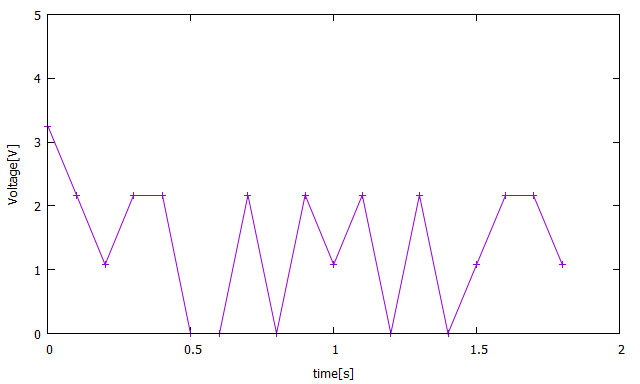
\includegraphics[width=7.0cm]{images/hatten2-4-1.png}
\caption{照度センサの値の変化}
\label{fig:hatten2-4-1}
\end{center}
\end{figure}



\section{発展課題2.4.2}
発展課題2.4.2において作成したスケッチと工夫点を報告せよ.また,照度センサの値の変化をグラフ化し,その結果を報告せよ.

以下ソースコード\ref{code:hatten2-4-2}に作成したスケッチを示す.

\begin{lstlisting}[caption = 発展課題2.4.2,label=code:hatten2-4-2][H]
const int LED1_PIN = 13; //13番ピンにLEDを接続
const int LED2_PIN = 9; //9番ピンにLEDを接続
int output = LOW;
int flag = 0;
unsigned long timePrev1 = 0; //基準となる時間を格納(10秒用)
unsigned long timePrev10 = 0; //基準となる時間を格納(10秒用)
unsigned long timePrev500 = 0; //基準となる時間を格納(500ms用)
unsigned long timePrev1000 = 0; //基準となる時間を格納(1000ms用)
void setup() {
  Serial.begin(9600); //シリアル通信を9600kbpsで初期化
  pinMode(LED1_PIN, OUTPUT); //13番ピンを出力ポートに設定
  pinMode(LED2_PIN,OUTPUT); //9番ピンを出力ポートに設定
}
void loop() { //ボーリング処理
  if((millis() - timePrev10) >= 10000){ //10秒経過
    timePrev10 = millis(); //時間情報の更新
    flag = 1; //10秒経過フラグ
  }
  if((millis() - timePrev500) >= 500){ //500ms経過
    output = !output; //出力を反転
    digitalWrite(LED1_PIN,output);
    timePrev500 = millis(); //時間情報の更新
  }
  if((millis() - timePrev1000) >= 1000){ //1000ms経過
    int sensorvalue = analogRead(A0); //A0ピンのAD変換結果を取得
    float vo = sensorvalue*(5.0/1024.0);
    float L =222*vo; //照度値に変換
    Serial.println(L); //シリアルモニタに表示
    delay(1); //安定用
    timePrev1000 = millis(); //時間の更新
    if ( flag == 1){ //10秒経過したら
      digitalWrite(LED2_PIN,HIGH); //LED2_PINを点灯させる
      flag = 0; //値を初期化
    }
    else { //そうでないなら
      digitalWrite(LED2_PIN,LOW); //LED2_PINは消灯
    }
  }
}
\end{lstlisting}

スケッチで工夫した点は,500ms,1000ms,10000ms経過用にそれぞれフラグを用意してそれぞれの秒数が経過したときに動作をするようにした.この動作はdelay関数を使わずにできたが自宅の開発環境ではSystem.println()のあとに安定用のdelayを用いないとエラーがでてしまったためそこだけdelay関数を使ってしまった.

また以下図\ref{fig:hatten2-4-1}に照度センサの値の変化のグラフを示す.

\begin{figure}[H]
\begin{center}
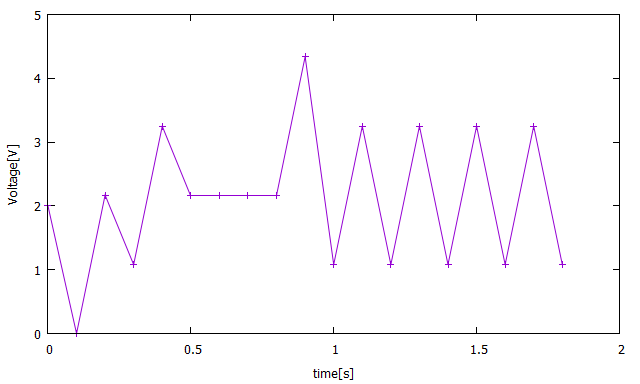
\includegraphics[width=7.0cm]{images/hatten2-4-2.png}
\caption{照度センサの値の変化}
\label{fig:hatten2-4-2}
\end{center}
\end{figure}

\section{発展課題2.4.3}
発展課題2.4.3において作成したスケッチと工夫点を報告せよ.

以下ソースコード\ref{code:hatten2-4-3}に作成したスケッチを示す.

\begin{lstlisting}[caption = 発展課題2.4.3,label=code:hatten2-4-3][H]
const int LED_PIN = 13; //LEDをD13に定義
const int SW_PIN = 2; //SWITCHをD2に定義
volatile int swnow = LOW; //現在の状態
volatile int swprev = LOW; //前の状態
unsigned long timePrev = 0; //基準となる時間を格納
volatile int output = LOW; //ディジタル出力の値を格納する変数:初期:LOW
/* 初期設定 */
void setup() {
  pinMode(LED_PIN,OUTPUT); //D13をディジタル出力に設定
  pinMode(SW_PIN,INPUT);
  /*外部割り込みの設定
    割り込みに使用するディジタルポートをD2に設定(1番目の引数="0")
    割り込みサービスルーチンblink関数を実行(2番目の引数=関数名)
    (例)割り込み要因としてスイッチの状態が"LOW"のときに発生(3番目の引数)
   */
   attachInterrupt(0,blink,FALLING);
}

void loop() {
  swprev = swnow;
  swnow = digitalRead(SW_PIN);
  if(swprev == LOW || swnow == HIGH){//ONからOFFになったとき
    timePrev = millis();
    while(millis() - timePrev >= 10){
      //10ms待つ
    }
  }
  digitalWrite(LED_PIN,output); //スイッチを押すたびに点灯・消灯を繰り返す
}

void blink() { //割り込みの条件にあわせLEDが点灯・消灯を繰り返す
  timePrev = millis();
  output = !output; //ディジタル出力を反転
  while(millis()-timePrev >= 10 ){
    //10ms待つ
  }
}
\end{lstlisting}

スケッチで工夫した点は,swprevとswnowを使ってONからOFF状態に推移した時とOFFからON状態に推移した時にチャタリング防止に10ms待つプログラムとしたところである.しかしながらこのプログラムでは入力に遅延が生じてしまうため,もう少し他の解決策も考えられる.

\end{document}
